% !TEX root = main.tex
\section{Evaluation in real-life contextual bandits}
\label{asec:evaluation_real_mab}

We evaluate the proposed method in two real-life bandit settings: \ie the recommendation of personalized news articles, and the optimal treatment selection strategy in precision oncology. The former represents an important example of reinforcement learning, as it requires efficient balancing of the exploration and exploitation tradeoff, and is here addressed in a similar fashion as done by~\citet{ic-Chapelle2011}. The latter is inspired by the work of~\citet{j-Rindtorff2019}, where they present a benchmark dataset to evaluate contextual bandit algorithms based on real in vitro drug responses of 896 cancer cell lines.

\subsection{Online content recommendation setting}
\label{ssec:evaluation_real_mab_yahoo}

We use the \href{https://webscope.sandbox.yahoo.com/catalog.php?datatype=r\&did=49}{R6A-Yahoo! Front Page Today Module User Click Log Dataset}, which contains user click logs for news articles displayed in the \textit{Featured Tab} of the \textit{Today Module on Yahoo! Front Page} during the first ten days in May 2009. The articles to be displayed were originally chosen uniformly at random from a hand-picked pool of high-quality articles. Here, we pick a subset of 23 articles shown in May 1st, with a total of 102,065 logged user interactions. We treat each article as an arm, $|\A|=23$, and the reward is whether the article is clicked or not by the user, $y_t=\{1,0\}$. The goal is to choose the most interesting article for each user, evaluated by counting the total number of clicks. In the dataset, each user is associated with six features, \ie the context $x_t\in\Real^{6}$: a bias term and five features that correspond to the membership features constructed via the conjoint analysis with a bilinear model described in~\citep{ip-Chu2009}. This problem is posed as a contextual MAB, where we want to maximize the click-through rate on the recommended articles for each user.

We provide results for the R6A-Yahoo! May 1st multi-armed bandit in Figure~\ref{fig:yahoo_showdown} and Table~\ref{tab:yahoo_showdown}. Note that, since the data was collected via a random allocation rule, we do not have access to the optimal algorithn (\ie the oracle that knows, for each user-article combination, what the most rewarding option would be). Accordingly, we present cumulative rewards of all the studied algorithms.

We observe that our proposed nonparametric Thompson sampling achieves performance comparable to alternatives that model expected rewards with linear regressors: \ie both the analytical \texttt{LinearGaussian TS} and the \texttt{NeuralLinear} baselines. In general, all studied methods show a very low reward ---signaling the complexity of the task at hand--- with a linear cumulative reward trend ---indicating they struggle to find the exploitation-exploration trade-off. Bootstrapped, RMS and dropout based neural networks show increased volatility in their otherwise best performance.

\begin{figure}[!h]
	\centering
	\begin{minipage}{0.45\textwidth}
		\includegraphics[width=\textwidth]{./figs/yahoo_may_01/cum_rewards_top_five_std}
		\caption{Mean cumulative rewards (standard deviation shown as shaded region) for 500 independent realizations of the presented methods in the R6A-Yahoo! May 1st MAB.}
		\label{fig:yahoo_showdown}
	\end{minipage}
	\qquad
	\begin{minipage}{0.48\textwidth}
		\centering
		\captionsetup{type=table}
		\resizebox*{\textwidth}{!}{
			\begin{tabular}{|c|c|}
				\hline
				Algorithm 	\cellcolor[gray]{0.6} & Total cumulative reward \cellcolor[gray]{0.6} \\ \hline
\texttt{Nonparametric TS}    	 & 49.895 $\pm$ 7.336 \\ \hline
\texttt{LinearGaussian TS}   	 & 49.923 $\pm$ 7.831 \\ \hline
\texttt{NeuralLinear}        	 & 50.393 $\pm$ 7.506 \\ \hline
\texttt{NeuralBootstrapped}  	 & 58.036 $\pm$ 10.037 \\ \hline
\texttt{NeuralRMS}           	 & 58.795 $\pm$ 10.539 \\ \hline
\texttt{NeuralDropoutRMS}    	 & 57.932 $\pm$ 11.367 \\ \hline
\texttt{NeuralParamNoise}    	 & 57.154 $\pm$ 9.432 \\ \hline
\texttt{MultitaskGP}        	 & 54.880 $\pm$ 9.545 \\ \hline
\texttt{BNNVariationalGaussian}	 & 55.870 $\pm$ 9.829 \\ \hline
\texttt{BNNAlphaDiv}        	 & 50.303 $\pm$ 8.429 \\ \hline
			\end{tabular}
		}
		\centering
		\caption{Final cumulative reward (mean and standard deviation) for 500 independent realizations of the presented methods in the in the R6A-Yahoo! May 1st MAB.}
		\label{tab:yahoo_showdown}
	\end{minipage}
\end{figure}

\subsection{Precision oncology setting}
\label{ssec:evaluation_real_mab_oncology}

We retrieve data from the following publicly available repository: \href{https://github.com/NiklasTR/oncoassign}{https://github.com/NiklasTR/oncoassign}. We collect in vitro drug response scores (after log-transformation and median centering of the original IC50 values), genomic features projected into a 20-dimensional manifold (cell-line specific features such as scaled gene expression data, binarized mutation and copy-number variant information were reduced to 20 dimensions by uniform manifold approximation and projection (UMAP)), as well as the manually curated seven therapeutic protocols. As in~\cite{j-Rindtorff2019}, these data is posed into a contextual MAB problem: the concatenation of the genomic low-dimensional UMAP features with the suggested therapeutic protocols forms the context per cell-line, the available actions are the seven possible treatments (afatinib, cisplatin, dabrafenib, olaparib, palbociclib, trametinib, vismodegib), and the observed rewards are the reversed in vitro drug response scores (since in its original form, the lowest response score is the strongest).

Results for the precision oncology dataset are provided in Figure~\ref{fig:precision_oncology_showdown} and Table~\ref{tab:precision_oncology_showdown}. We observe that the proposed nonparametric Thompson sampling achieves performance similar to that of the analytical \texttt{LinearGaussian TS} alternative, with reduced regret when compared to the \texttt{NeuralLinear} Thompson sampling. As in previous scenarios, Gaussian process based methods suffer in these real-data MABs (see Tables~\ref{tab:yahoo_showdown} and Tables~\ref{tab:precision_oncology_showdown}), as determining which Gaussian process mean and kernel functions to use is critical, yet arduous.

For the studied methods, the regret curve is sublinear, with slightly better (yet very volatile) performance achieved by bootstrapped, RMS, and noise injection based neural network baselines. These methods that rely on extrinsic randomness offer average improvements in these real-life datasets, with considerably (2 to 3 times) higher volatility than the proposed nonparametric method.

\begin{figure}[!h]
	\centering
	\begin{minipage}{0.45\textwidth}
		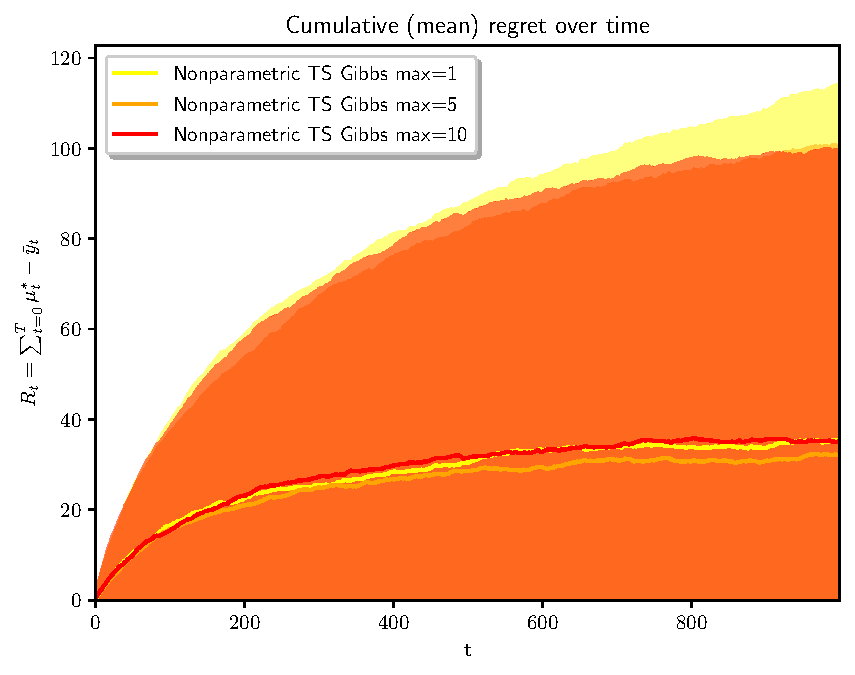
\includegraphics[width=\textwidth]{./figs/precision_oncology/cum_optexpected_regret_top_five_std}
		\caption{Mean regret (standard deviation shown as shaded region) for 500 independent realizations of the presented methods in the precision oncology MAB.}
		\label{fig:precision_oncology_showdown}
	\end{minipage}
	\qquad
	\begin{minipage}{0.48\textwidth}
		\centering
		\captionsetup{type=table}
		\resizebox*{\textwidth}{!}{
			\begin{tabular}{|c|c|}
				\hline
				Algorithm 	\cellcolor[gray]{0.6} & Total cumulative reward \cellcolor[gray]{0.6} \\ \hline
\texttt{Optimal} 	 	 	 & 1998.238 $\pm$ 0.000 \\ \hline
\texttt{Nonparametric TS}     	 & 705.219 $\pm$ 53.038 \\ \hline
\texttt{LinearGaussian TS}   	 & 709.351 $\pm$ 52.132 \\ \hline
\texttt{NeuralLinear}        	 & 633.900 $\pm$ 59.682 \\ \hline
\texttt{NeuralBootstrapped}  	 & 752.509 $\pm$ 114.593 \\ \hline
\texttt{NeuralRMS}           	 & 712.567 $\pm$ 151.703 \\ \hline
\texttt{NeuralDropoutRMS}    	 & 704.339 $\pm$ 150.107 \\ \hline
\texttt{NeuralParamNoise}    	 & 739.107 $\pm$ 124.098 \\ \hline
\texttt{MultitaskGP}         	 & 513.204 $\pm$ 66.543 \\ \hline
\texttt{BNNVariationalGaussian}	 & 611.194 $\pm$ 155.471 \\ \hline
\texttt{BNNAlphaDiv}         	 & 327.344 $\pm$ 53.567 \\ \hline
			\end{tabular}
		}
		\centering
		\caption{Final cumulative reward (mean and standard deviation) for 500 independent realizations of the presented methods in the precision oncology MAB.}
		\label{tab:precision_oncology_showdown}
	\end{minipage}
\end{figure}
